\begin{tikzpicture}[x=1mm, y=1mm, font=\footnotesize,
    bloque/.style={draw, rounded corners, align=center, minimum height=9mm,
                   minimum width=24mm, font=\footnotesize, inner xsep=1mm},
    modelo/.style={bloque, fill=miaamarillo!30},
    proc/.style={bloque, fill=black!5, minimum width=26mm},
    salida/.style={bloque, fill=green!12, minimum width=16mm},
    flecha/.style={-{Latex[length=2mm]}, thick},
    etiq/.style={font=\scriptsize, align=center, inner sep=0.3mm},
    % pila de K vectores de probabilidad (icono)
    pics/probvec/.style={code={
      \foreach \d in {2.0,1.0} {\draw[fill=white, thin] (\d,\d) rectangle ++(9,6);}
      \draw[fill=white, thin] (0,0) rectangle (9,6);
      \foreach \bx/\bh in {0.9/1.2, 2.2/0.7, 3.5/4.6, 4.8/1.0, 6.1/1.9, 7.4/0.8}
        {\fill[pucazul!80] (\bx,0.5) rectangle ++(1.0,\bh);}
    }}]

  % ================= (a) AUDIO =================
  \node[anchor=west, inner sep=0] at (0,7.5)
    {\textbf{(a)} Audio: grabación de \SI{45}{s} a \SI{32}{kHz}};
  % barra de la grabación (45 mm = 45 s) con forma de onda estilizada
  \begin{scope}
    \draw[fill=pucazul!15, thin, rounded corners=0.8mm] (0,-3.5) rectangle (45,3.5);
    \clip (0,-3.5) rectangle (45,3.5);
    \draw[pucazul!60!black, line width=0.3pt]
      plot[domain=0:45, samples=320, smooth]
      (\x, {(0.22 + 2.7/(1+((\x-10)/2.2)^2) + 2.2/(1+((\x-24)/1.8)^2)
            + 2.0/(1+((\x-37)/1.6)^2)) * (0.7+0.3*sin(\x*73)) * sin(\x*300)});
  \end{scope}
  % K = 9 ventanas contiguas de 5 s (5 mm cada una)
  \foreach \i in {0,...,8} {
    \draw[fill=black!5, thin] ({\i*5},-8) rectangle ({\i*5+5},-4.5);
  }
  \draw[fill=miaamarillo!30, thick] (20,-8) rectangle (25,-4.5);
  \node[etiq, anchor=north west, align=left] at (0,-9.3)
    {$W=9$ ventanas de \SI{5}{s}, equiespaciadas ($W\le 12$)\\
     amarillo: \emph{ventana única} (central)};

  % pipeline (a), centrado en y=-2
  % llave: cada una de las K ventanas (no la grabación entera) entra a la CNN
  \draw[decorate, decoration={brace, amplitude=1.2mm}, thin] (46,3.5) -- (46,-8);
  \node[modelo] (cnn) at (72.5,-2) {CNN de audio\\EfficientNet-B0\\+ softmax};
  \draw[flecha] (48.2,-2.25) -- (cnn.west |- 0,-2.25)
    node[midway, above=0.4mm, etiq] {log-mel}
    node[midway, below=0.4mm, etiq] {$128{\times}501$};
  \pic at (88,-6.5) {probvec};
  \node[etiq, anchor=north] at (93.5,-7.6) {$W$ vectores\\$p^{(w)}\in\mathbb{R}^{55}$};
  \draw[flecha] (cnn.east) -- (87.6,-2);
  \node[proc] (prom) at (117.5,-2) {Promedio\\$\bar{p}=\frac{1}{W}\sum_{w} p^{(w)}$};
  \draw[flecha] (100.4,-2) -- (prom.west);
  \node[salida] (esp) at (149,-2) {Especie\\$\hat{y}$};
  \draw[flecha] (prom.east) -- (esp.west) node[midway, above=0.4mm, etiq] {$\arg\max$};

  % ================= (b) IMAGEN =================
  \node[anchor=west, inner sep=0] at (0,-23)
    {\textbf{(b)} Imagen: fotografía redimensionada (lado menor a \SI{441}{px})};
  % fotografía real del corpus (chucao, iNaturalist, CC BY-NC 4.0), recortada a 28 x 21 mm
  \begin{scope}
    \clip (8,-46.5) rectangle (36,-25.5);
    \node[inner sep=0] at (22,-36) {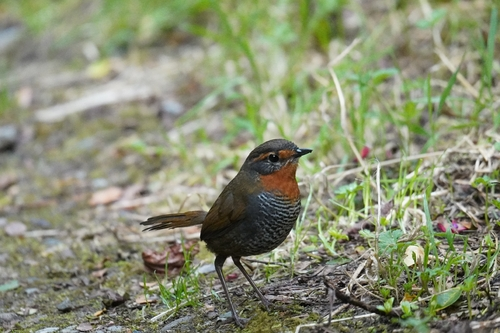
\includegraphics[height=21mm]{fig_tta_foto.jpg}};
  \end{scope}
  \draw[thin, black!40] (8,-46.5) rectangle (36,-25.5);
  % 4 recortes de esquina (azul, discontinuo): cuadrados de 15 x 15 mm, solapados
  \foreach \px/\py in {8/-25.5, 21/-25.5, 8/-31.5, 21/-31.5} {
    \draw[pucazul!70!black, dash pattern=on 1.2pt off 0.9pt, line width=0.5pt]
      (\px,\py) rectangle ++(15,-15);
  }
  % recorte central (amarillo, continuo), cuadrado de 15 x 15 mm
  \draw[miaamarillo!80!black, thick] (14.5,-28.5) rectangle ++(15,-15);
  \node[etiq, anchor=north west, align=left] at (0,-47.8)
    {5 recortes de $384{\times}384$ px: 4 esquinas + centro\\
     amarillo: \emph{recorte central} (1 vista)};

  % pipeline (b), centrado en y=-36
  \node[modelo] (b3) at (72.5,-36) {CNN de imagen\\EfficientNet-B3\\+ softmax};
  \draw[flecha] (36.4,-36) -- (b3.west)
    node[midway, above=0.4mm, etiq] {$\times 2$ volteo\\horizontal}
    node[midway, below=0.4mm, etiq] {$= 10$ vistas};
  \pic at (88,-40.5) {probvec};
  \node[etiq, anchor=north] at (93.5,-41.6) {10 vectores\\$p^{(v)}\in\mathbb{R}^{53}$};
  \draw[flecha] (b3.east) -- (87.6,-36);
  \node[proc] (promb) at (117.5,-36) {Promedio (TTA)\\$\bar{p}=\frac{1}{10}\sum_{v} p^{(v)}$};
  \draw[flecha] (100.4,-36) -- (promb.west);
  \node[salida] (espb) at (149,-36) {Especie\\$\hat{y}$};
  \draw[flecha] (promb.east) -- (espb.west) node[midway, above=0.4mm, etiq] {$\arg\max$};
\end{tikzpicture}
